\documentclass[11pt, a4paper, twoside]{article}   	% use "amsart" instead of "article" for AMSLaTeX format

\usepackage{geometry}                		% See geometry.pdf to learn the layout options. There are lots.
\usepackage{pdfpages}
\usepackage{caption}
\usepackage{minted}
\usepackage[german]{babel}			% this end the next are needed for german umlaute
\usepackage[utf8]{inputenc}
\usepackage{color}
\usepackage{graphicx}
\usepackage{titlesec}
\usepackage{fancyhdr}
\usepackage{lastpage}
\usepackage{hyperref}
\usepackage[autostyle=false, style=english]{csquotes}
\usepackage{mathtools}
\usepackage{tabularx}
% http://www.artofproblemsolving.com/wiki/index.php/LaTeX:Symbols#Operators
% =============================================
% Layout & Colors
% =============================================
\geometry{
   a4paper,
   total={210mm,297mm},
   left=20mm,
   right=20mm,
   top=20mm,
   bottom=30mm
 }	

\definecolor{myred}{rgb}{0.8,0,0}
\definecolor{mygreen}{rgb}{0,0.6,0}
\definecolor{mygray}{rgb}{0.5,0.5,0.5}
\definecolor{mymauve}{rgb}{0.58,0,0.82}

\setcounter{secnumdepth}{4}


% the default java directory structure and the main packages
\newcommand{\srcDirGenerator}{../src/T4/ClassGenerator}
\newcommand{\srcDirClone}{../src/T4/CloningGenerator}
\newcommand{\srcDirJavaSrc}{../src/gp2.svg-generator/src/main/java}
\newcommand{\srcDirJavaRes}{../src/gp2.svg-generator/src/main/resources}
\newcommand{\imageDir}{images}
% =============================================
% Code Settings
% =============================================
\newenvironment{code}{\captionsetup{type=listing}}{}
\newmintedfile[cppSourceFile]{cpp}{
	linenos=true, 
	frame=single, 
	breaklines=true, 
	tabsize=2,
	numbersep=5pt,
	xleftmargin=10pt,
	baselinestretch=1,
	fontsize=\footnotesize
}
\newmintedfile[xmlFile]{xml}{
	linenos=true, 
	frame=single, 
	breaklines=true, 
	tabsize=2,
	numbersep=5pt,
	xleftmargin=10pt,
	baselinestretch=1,
	fontsize=\footnotesize
}
\newmintedfile[jsonFile]{json}{
	linenos=true, 
	frame=single, 
	breaklines=true, 
	tabsize=2,
	numbersep=5pt,
	xleftmargin=10pt,
	baselinestretch=1,
	fontsize=\footnotesize
}
\newmintinline[inlineCpp]{cpp}{}
\newminted[cppSource]{cpp}{
	breaklines=true, 
	tabsize=2,
	autogobble=true,
	breakautoindent=false
}

\newcommand{\xvdash}[1]{%
  \vdash^{\mkern-10mu\scriptscriptstyle\rule[-.9ex]{0pt}{0pt}#1}%
}

% =============================================
% Page Style, Footers & Headers, Title
% =============================================
\title{Übung 3}
\author{Thomas Herzog}

\lhead{Übung 3}
\chead{}
\rhead{
\includegraphics[scale=0.10]{FHO_Logo_Students.jpg}}

\lfoot{S1610454013}
\cfoot{}
\rfoot{ \thepage / \pageref{LastPage} }
\renewcommand{\footrulewidth}{0.4pt}
% =============================================
% D O C U M E N T     C O N T E N T
% =============================================
% =============================================
% 2016.10.13: 1 
% 2016.10.14: 2
% =============================================
\pagestyle{fancy}
\begin{document}
\setlength{\headheight}{15mm}
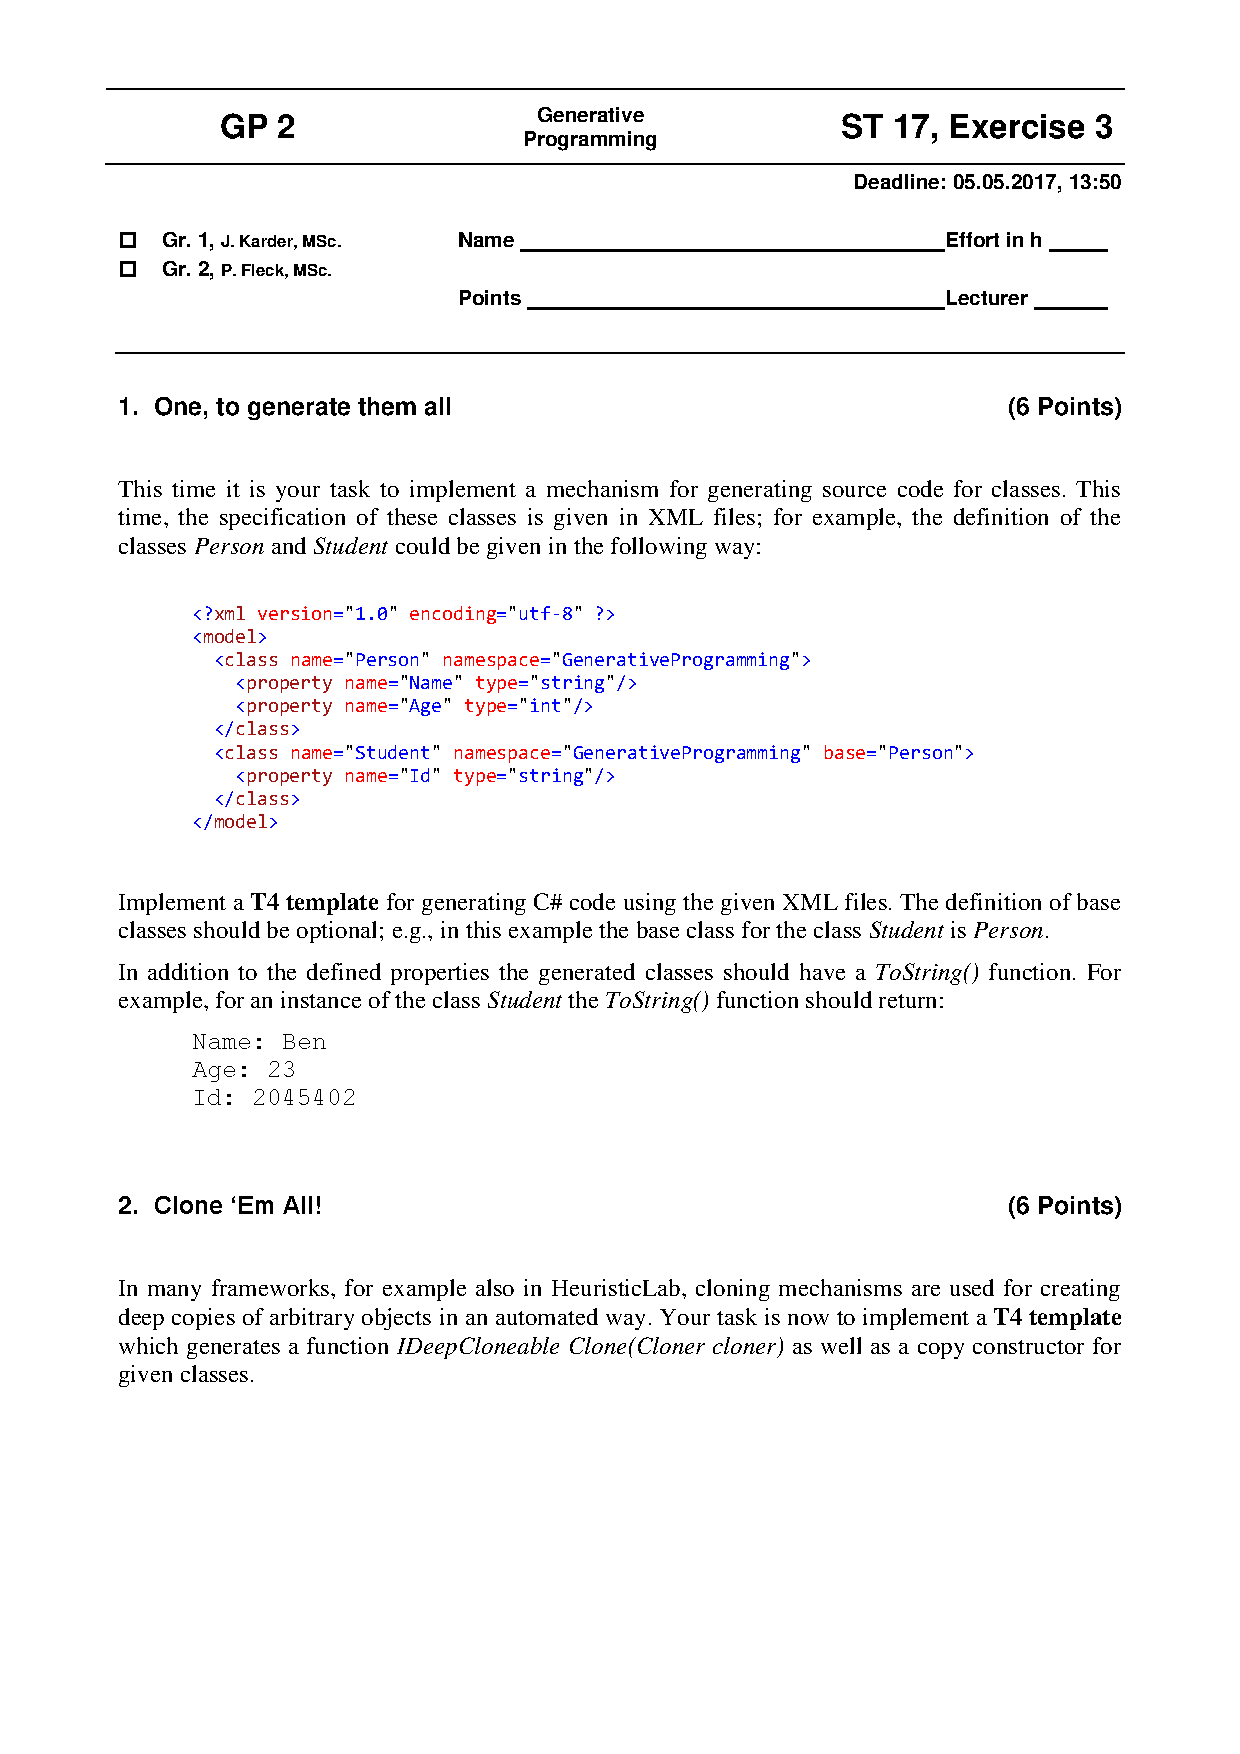
\includepdf[pages={1,2,3,4,5}]{GP_A03.pdf}

\section{One, to generate them all}
\subsection{Lösungsidee}
Dieser Abschnitt beschäftigt sich mit der Dokumentation der Lösungsidee der Aufgabenstellung \emph{One, to generate them all}. Um von den \emph{XML-Tag}-Namen und dessen Attributen unabhängig zu sein sollen die \emph{XML-Tag}-Namen und dessen Attribute in Konstanten ausgelagert werden und sollen bei der Navigation durch das \emph{XML}-Dokument verwendet werden, um die \emph{XML-Tags} sowie dessen Attribute zu adressieren. Die Unabhängigkeit von der Struktur des \emph{XML}-Dokuments ist aber nicht möglich.
\newline
\newline
Da die im \emph{XML}-Dokument definierten Klassen sich im selben Namensraum befinden können,  sollen die definierten Klassen nach den Namensräumen gruppiert werden, damit die Namensräume nicht mehrfach in den generierten Klassen definiert werden müssen. Um das zu realisieren soll \emph{Linq} verwendet werden. Um sich zu viele \emph{If}-Blöcke im \emph{T4-Template} zu vermeiden soll mit dem \emph{?} Operator gearbeitet werden, um die resultierenden Zeichenketten des \emph{C\#}-Quelltextes zu generieren. Dadurch soll das \emph{T4-Template} übersichtlicher werden, da meiner Meinung nach das Verwenden von zu vielen \emph{If}-Anweisungen das \emph{Template} unübersichtlich macht.
\newline
\newline
Zusätzlich zu den verlangten Attributen der \emph{XML-Tags} wurde noch auf Klassenebene ein \emph{Modifier} eingeführt, womit auch abstrakte Klassen möglich sind.  
\newline
\newline
Die \emph{Tostring} Methode wurde so implementiert, dass wenn es eine Basisklasse gibt, zuerst an diese Basisklasse delegiert wird und dann erst die Ausgabe der konkreten Klasse erfolgt, wobei am Anfang einer jeder \emph{Tostring} Implementierung immer die der Klassennamen ausgegeben wird.     

\subsection{Quelltexte}
Folgender Abschnitt enthält die Quelltexte der Aufgabenstellung.
\begin{code}
	\caption{ClassGenerator.tt}
	\cppSourceFile{\srcDirGenerator/ClassGenerator.tt}
	\label{src:class-generator-tt}
\end{code}

\begin{code}
	\caption{Model.xml}
	\xmlFile{\srcDirGenerator/Model.xml}
	\label{src:model-xml}
\end{code}

\begin{code}
	\caption{Program.cs}
	\cppSourceFile{\srcDirGenerator/Program.cs}
	\label{src:program-cs}
\end{code}

\subsection{Tests}
Folgender Abschnitt enthält die Tests der Aufgabenstellung in Form der generierten Quelltexte sowie der Ausgaben des Testprogramms.

\begin{code}
	\caption{ClassGenerator.cs}
	\cppSourceFile{\srcDirGenerator/ClassGenerator.cs}
	\label{src:class-generator-cs}
\end{code}
\ \newpage

\begin{figure}[h]
	\centering
	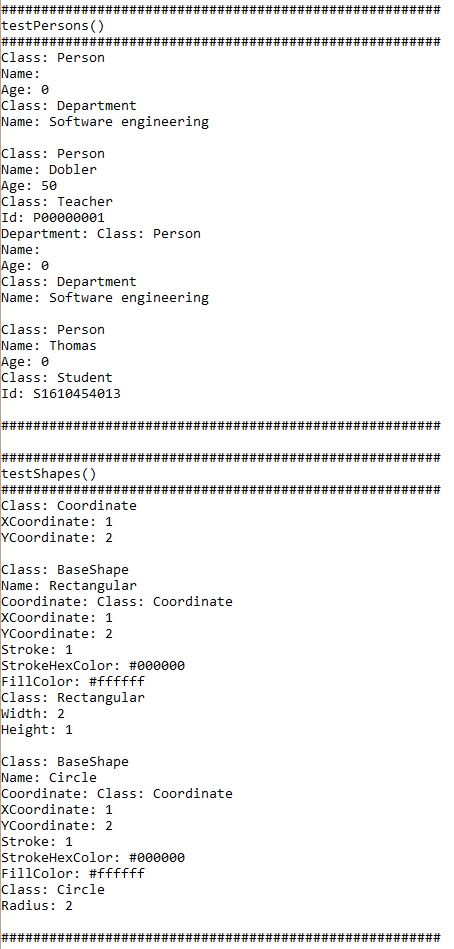
\includegraphics[scale=0.73]{\imageDir/class-generator.JPG}
	\caption{\emph{Class} Generator Testausgabe}
	\label{fig:class-generator}
\end{figure}
\ \newpage

\section{Clone 'Em All}
\subsection{Lösungsidee}
Dieser Abschnitt beschäftigt sich mit der Dokumentation der Lösungsidee der Aufgabenstellung \emph{Clone 'Em All}. Diese Aufgabenstellung wurde bereits in der Übung implementiert und nachträglich formatiert und einige Kommentare eingefügt.

\subsection{Quelltexte}
In diesem Abschnit werden nur die selbst implementierten Quelltexte angeführt.

\begin{code}
	\caption{CloningGenerator.tt}
	\cppSourceFile{\srcDirClone/CloningGenerator.tt}
	\label{src:cloning-generator-tt}
\end{code}

\begin{code}
	\caption{A.cs}
	\cppSourceFile{\srcDirClone/A.cs}
	\label{src:a-cs}
\end{code}

\begin{code}
	\caption{B.cs}
	\cppSourceFile{\srcDirClone/B.cs}
	\label{src:b-cs}
\end{code}

\begin{code}
	\caption{Program.cs}
	\cppSourceFile{\srcDirClone/Program.cs}
	\label{src:cloning-program-cs}
\end{code}

\subsection{Tests} 
Dieser Abschnitt enthält die Tests in Form von den generierten Quelltexten und der Ausgabe des Testprogramms.

\begin{code}
	\caption{CloningGenerator.cs}
	\cppSourceFile{\srcDirClone/CloningGenerator.cs}
	\label{src:cloning-generator-cs}
\end{code}

\begin{figure}[h]
	\centering
	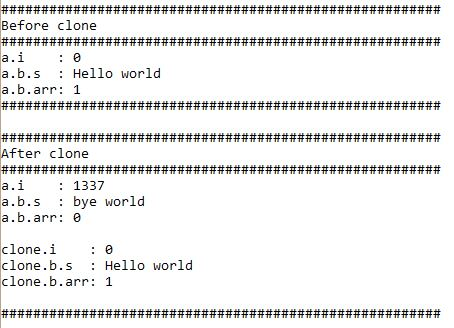
\includegraphics[scale=0.73]{\imageDir/clone-generator.JPG}
	\caption{\emph{Clone} Generator Testausgabe}
	\label{fig:clone-generator}
\end{figure}

\section{SVG Generator}
Dieser Abschnitt beschäftigt sich mit der Dokumentation der Lösungsidee der Aufgabenstellung \emph{SVG Generator}.

\subsection{Lösungsidee}

\subsection{Quelltexte}

\subsection{Tests}

\end{document}